%===
\subsection{1(a)}
Four rectangular parallelopipeds, A, B, C, and D, are arranged as shown in Figure~\ref{1_a}.
$\pmb a_1, \pmb a_2, \pmb a_3$ designate unit vedtors respectively parallel to the edges of $A$: $\pmb b_1, \pmb b_2, \pmb b_3$ are unit vectors respectively parallel to the edges of $B$, and so forth, and $\phi, \theta$ and $\psi$ denote the radian measures of angles that determine the relative orientiation of the bodies.
The configuration shown is one in which $\phi, \theta, \psi$ are regarded positive. Determine the maginitude of each of the following derivatives:

\begin{align*}
  \lx{^B}{\frac {\partial \pmb a_1}  {\partial \phi}}, \:
  \lx{^B}{\frac {\partial \pmb b_1}  {\partial \phi}}, \:
  \lx{^B}{\frac {\partial \pmb a_3}  {\partial \phi}}, \:
  \lx{^B}{\frac {\partial \pmb b_2}  {\partial \theta}}, \:
  \lx{^C}{\frac {\partial \pmb b_2}  {\partial \theta}}, \:
  \lx{^D}{\frac {\partial \pmb b_2}  {\partial \theta}}, \:
  \lx{^C}{\frac {\partial \pmb b_2}  {\partial \psi}}, \:
  \lx{^D}{\frac {\partial \pmb b_2}  {\partial \psi}}, \:
  \lx{^D}{\frac {\partial \pmb a_1}  {\partial \psi}}
\end{align*}

\begin{figure}[H]
    \centering
    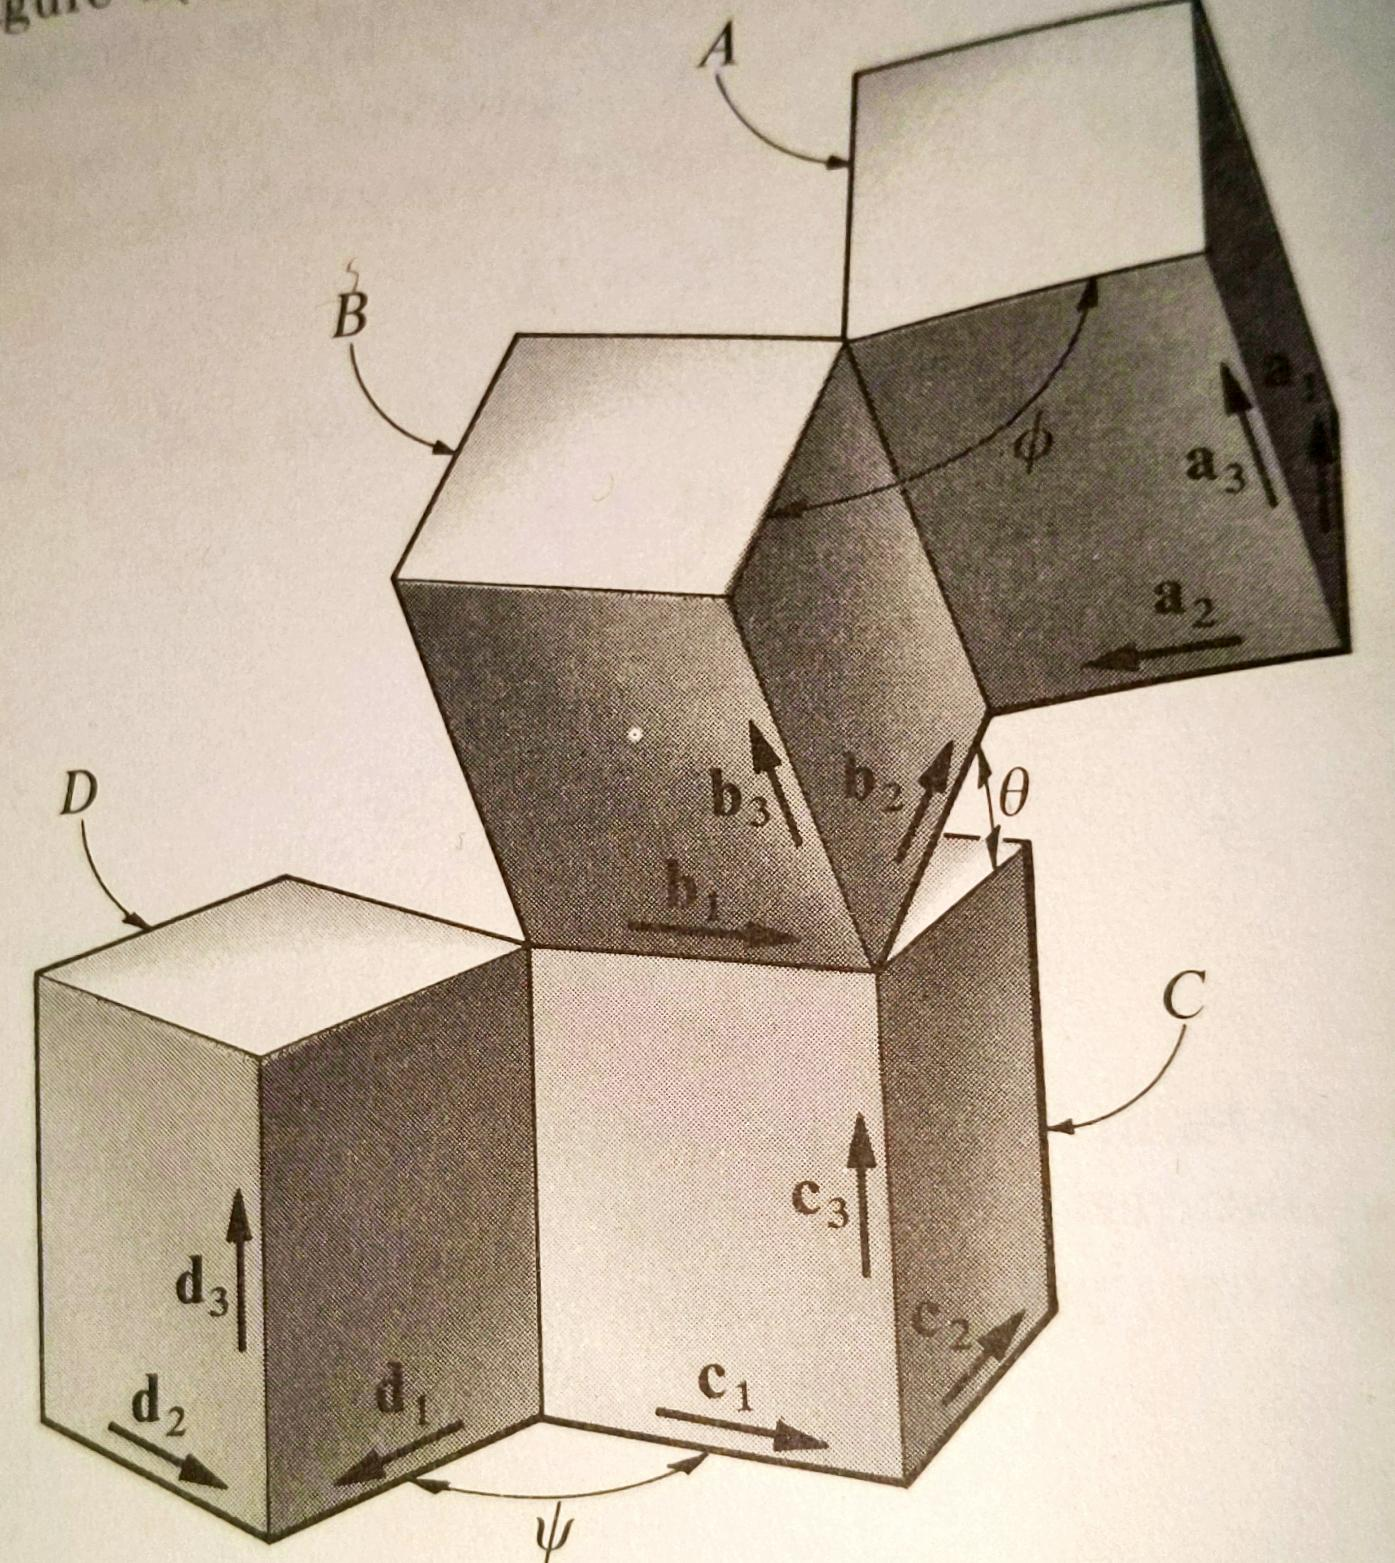
\includegraphics[width = 0.5\textwidth, height = 0.5\textwidth]{./figs/ProbSet_1/1_a.jpg}
    \caption{}
    \label{1_a}
\end{figure}


\textbf{\textit{sol.}}\\

We have the following rotation matrices:

\begin{align*}
     &\lx{^B}{\bm{\pmb a_1 \\ \pmb a_2 \\ \pmb a_3}} =
     \underbrace{
        \bm{
            \cos \phi & \sin \phi  & 0\\
            -\sin \phi & \cos \phi & 0\\
            0          & 0         & 1
        }
     } _ {R_3 (\phi)}
    \lx{^B}{\bm{\pmb b_1 \\ \pmb b_2 \\ \pmb b_3}} ;\:
    %===
    \lx{^C}{\bm{\pmb b_1 \\ \pmb b_2 \\ \pmb b_3}} =
    \underbrace{
        \bm{
            1 & 0 & 0\\
            0 & \cos \theta & \sin \theta\\
            0 & -\sin \theta & \cos \theta
        }
     } _ {R_1 (\theta)}
    \lx{^C}{\bm{\pmb c_1 \\ \pmb c_2 \\ \pmb c_3}} ;\:
    %===
    \lx{^D}{\bm{\pmb c_1 \\ \pmb c_2 \\ \pmb c_3}} =
     \underbrace{
        \bm{
            \cos \psi & \sin \psi  & 0\\
            -\sin \psi & \cos \psi & 0\\
            0          & 0         & 1
        }
     } _ {R_3 (\psi)}
    \lx{^D}{\bm{\pmb d_1 \\ \pmb d_2 \\ \pmb d_3}} \\
    %===
    &\text{Let, } \qquad
    \pmb a = \bm{\pmb a_1 \\ \pmb a_2 \\ \pmb a_3} \quad
    \pmb b = \bm{\pmb b_1 \\ \pmb b_2 \\ \pmb b_3} \quad
    \pmb c = \bm{\pmb c_1 \\ \pmb c_2 \\ \pmb c_3} \quad
    \pmb d = \bm{\pmb d_1 \\ \pmb d_2 \\ \pmb d_3}
\end{align*}

Thus, we have,

\begin{enumerate}
 \item
 \begin{align*}
   \lx{^B}{\frac {\partial \pmb a_1}  {\partial \phi}}&=
   %=
   \frac{\partial}{\partial \phi} \left(R_3(\phi)[1, :]  \times \lx{^B}{\pmb b} \right)
   %=
   = \frac{\partial R_3(\phi)[1, :]}{\partial \phi} \lx{^B}{\pmb b}
   %=
   \qquad \left[\because \pmb b_1, \pmb b_2,  \pmb b_3
   \text{ are fixed in } B \right]\\
   %=
   &= \bm{-\sin \phi & cos \phi & 0}
    \times \lx{^B}{\pmb b}\\
    %===
    &\implies \lx{^B}{\norm{\frac {\partial \pmb a_1}  {\partial \phi}}} = 1
 \end{align*}

 \item
 \begin{align*}
    \lx{^B}{\frac {\partial \pmb b_1}  {\partial \phi}} &= 0
    %=
    \implies \lx{^B}{\norm{ \frac {\partial \pmb b_1}  {\partial \phi}}} = 0
    %=
   \qquad \left[\because \pmb b_1, \pmb b_2,  \pmb b_3
   \text{ are fixed in } B \right]\\
 \end{align*}

 \item
 \begin{align*}
    \lx{^B}{\frac {\partial \pmb a_3}  {\partial \phi}} &=
   %=
   \frac{\partial}{\partial \phi} \left(R_3(\phi)[3, :]  \times \lx{^B}{\pmb b} \right)
   %=
   = \frac{\partial \pmb b_3}{\partial \phi}
   = 0
   %=
   \qquad \left[\because \pmb b_1, \pmb b_2,  \pmb b_3
   \text{ are fixed in } B \right]\\
   %===
   &\implies \lx{^B}{\norm{\frac {\partial \pmb a_3}  {\partial \phi}}} = 0
 \end{align*}


 \item
 \begin{align*}
    \lx{^B}{\frac {\partial \pmb b_2}  {\partial \theta}} &= 0
    \implies \lx{^B}{\norm{\frac {\partial \pmb b_2}  {\partial \theta}}} = 0
    \qquad \left[\because \pmb b_1, \pmb b_2,  \pmb b_3
   \text{ are fixed in } B \right]\\
 \end{align*}

\item
\begin{align*}
    \lx{^C}{\frac {\partial \pmb b_2}  {\partial \theta}} &= \frac {\partial}  {\partial \theta} \left( R_1(\theta)[2,:] \times \lx{^C}{\pmb c} \right)
    = \frac{\partial R_1(\theta)[2,:]}{\partial \theta} \times \lx{^C}{\pmb c}
    \qquad \left[\because \pmb c_1, \pmb c_2, \pmb c_3 \text{ are fixed in } C \right]\\
    %==
    &= \bm{0 & -\sin \theta & \cos \theta} \times \lx{^C}{\pmb c}\\
    %===
    &\implies \lx{^C}{\norm{\frac {\partial \pmb b_2}  {\partial \theta}}} = 1
\end{align*}


 \item
 \begin{align*}
    \lx{^D}{\frac {\partial \pmb b_2}  {\partial \theta}} &= \frac {\partial}  {\partial \theta} \left((R_1(\theta) R_3(\psi))[2,:] \times \lx{^D}{\pmb d} \right)
    \qquad \left[\because \pmb d_1, \pmb d_2, \pmb d_3 \text{ are fixed in } D \right]\\
    %===
    &= \frac{\partial (R_1(\theta) R_3(\psi))[2,:]}{\partial \theta} \lx{^D}{\bm{\pmb d_1 \\ \pmb d_2 \\ \pmb d_3}}
    %===
    = \left(\frac{\partial R_1(\theta) }{\partial \theta} R_3(\psi) \right) [2,:]\lx{^D}{\pmb d}
    %===
    = \left(\frac{\partial R_1(\theta)[2,:] }{\partial \theta} R_3(\psi) \right)\lx{^D}{\pmb d}\\
    %===
    &=  \left( \bm{0 & -\sin \theta & \cos \theta}
    \bm{
            \cos \psi & \sin \psi  & 0\\
            -\sin \psi & \cos \psi & 0\\
            0          & 0         & 1
        } \right)\lx{^D}{\pmb d}
    %===
    = \bm{\sin \theta \sin \psi & -\sin \theta \cos \psi & \cos \theta} \lx{^D}{\pmb d}\\
    %===
    &\implies  \lx{^D}{\norm{\frac {\partial \pmb b_2}  {\partial \theta}}} = 1
 \end{align*}

 \item
\begin{align*}
    \lx{^C}{\frac {\partial \pmb b_2}  {\partial \psi}} &= 0
    \implies \lx{^C}{\norm{\frac {\partial \pmb b_2}  {\partial \psi}}} = 0
    \qquad \left[ \because \text{Any vector defined in C is independent of } \psi \right]
\end{align*}

 \item
\begin{align*}
    \lx{^D}{\frac {\partial \pmb b_2}  {\partial \psi}} &= \frac{\partial}{\partial \psi} \left((R_1(\theta) R_3(\psi))[2,:] \times \lx{^D}{\pmb d} \right)
    \qquad \left[\because \pmb d_1, \pmb d_2, \pmb d_3 \text{ are fixed in } D \right]\\
    %==
    &= R_1(\theta)[2,:] \times \frac{\partial R_3(\psi)}{\partial \psi} \times \lx{^D}{\pmb d}
    %==
    = \bm{0 & \cos \theta & \sin \theta} \bm{-\sin \psi & \cos \psi & 0 \\
                                             -\cos \psi & -\sin \psi & 0\\
                                             0 & 0 & 0}
                        \times \lx{^D}{\pmb d}\\
    %==
    &= \bm{-\cos \theta \cos \psi & -\cos \theta \sin \psi & 0} \times \lx{^D}{\pmb d}\\
    %==
    &\implies  \lx{^D}{\norm{\frac {\partial \pmb b_2}  {\partial \psi}}} = \norm{\cos \theta}
\end{align*}

\item
\begin{align*}
    \lx{^D}{\frac {\partial \pmb a_1}  {\partial \psi}} &=  \frac{\partial}{\partial \psi} \left((R_3(\phi)R_1(\theta) R_3(\psi))[2,:] \times \lx{^D}{\pmb d} \right)
    %==
    = R_3(\phi)[1,:] \times R_1(\theta) \times \frac{\partial R_3(\psi)}{\partial \psi} \times \lx{^D}{\pmb d}\\
    %==
    %\quad \left[\because \pmb d_1, \pmb d_2, \pmb d_3 \text{ are fixed in } D \right]\\
    %==
    &= \bm{\cos \phi & \sin \phi  & 0}
      \bm{
            1 & 0 & 0\\
            0 & \cos \theta & \sin \theta\\
            0 & -\sin \theta & \cos \theta
        }
      \bm{
            -\sin \psi & \cos \psi  & 0\\
            -\cos \psi & -\sin \psi & 0\\
            0          & 0         & 0
        }\lx{^D}{\pmb d}\\
    %==
    &= \bm{-\cos \phi \sin \psi - \sin \phi \cos \theta \cos \psi &
          \cos \phi \cos \psi - \sin \phi \cos \theta \sin \psi &
          0} \lx{^D}{\pmb d}\\
    %==
     \implies \lx{^D}{\norm{\frac {\partial \pmb a_1}  {\partial \psi}}} &=
    \sqrt{(-\cos \phi \sin \psi - \sin \phi \cos \theta \cos \psi )^2 +
    (\cos \phi \cos \psi - \sin \phi \cos \theta \sin \psi )^2}\\
    %==
    &= (\cos^2 \phi + \sin^2\phi \sin^2 \theta)^{1/2}
\end{align*}

\end{enumerate}
